\documentclass[12pt,oneside]{article}
\usepackage{makeidx,anysize,mflogo,xspace,float,epsfig,url}
\usepackage{amsmath,amsfonts,amssymb,a4wide} 
\usepackage[utf8]{inputenc}
\usepackage[french]{babel}
\urlstyle{sf}
\usepackage{hyperref}
\usepackage{graphicx}
\usepackage{graphics}
\usepackage{float}
\usepackage{caption}
\usepackage{colordvi} %??
\usepackage{listings} 
\usepackage{subfigure}
\usepackage{subfloat}
\usepackage{xcolor}
%\usepackage[labelsep=quad,indention=10pt]{subfig}
\definecolor{grey}{rgb}{0.95,0.95,0.95} % on définit la couleur grise
	% (c'est un gris très clair)
	\definecolor{red}{rgb}{1.0,0.0,0.0} 
	\definecolor{green}{rgb}{0.0,1.0,0.0}
	\definecolor{blue}{rgb}{0.0,0.0,1.0}
	\lstloadlanguages{bash,Java,C,C++,csh,make,sh}%%[Visual]Basic,xml}
	\lstset{frame=none,basicstyle=\footnotesize,breaklines,tabsize=2,captionpos=b,
		prebreak={\hbox{$\rightarrow$}},postbreak={\hbox{$\hookrightarrow$}},
		showstringspaces=false,backgroundcolor=\color{grey}\bfseries,
		keywordstyle=\color{blue},commentstyle=\color{green}\textit,
		stringstyle=\color{red}\ttfamily,abovecaptionskip=2pt,aboveskip=0pt,
		belowskip=0pt,belowcaptionskip=0pt,numbers=none,columns=fullflexible, backgroundcolor=\color{grey}}
%left,numberstyle=\footnotesize,
%		stepnumber=2,numbersep=1pt}
\graphicspath{{./figures/}}

\begin{document}


\begin{center}
{\bf \Large Redpitaya~: Premier exemple de projet Vivado ADC et DAC} \\ \ \\
G. Goavec-M\'erou \\ \ \\ \today
\end{center}

Ce document a pour but de fournir les bases pour~:
\begin{itemize}
\item la cr\'eation d'un projet dans {\tt Vivado} et de son bloc design associ\'e;
\item l'ajout d'IPs et les connexions tant, entre elles, que sur les broches du
FPGA;
\item la g\'en\'eration du bitstream;
\item la conversion de ce dernier et la programmation du FPGA.
\end{itemize}

Cette pr\'esentation va consister en l'utilisation de l'ADC et du DAC
pr\'esent sur la carte {\tt redpitaya}, ainsi qu'au branchement de la sortie de
l'ADC sur l'entr\'ee du DAC (mode dit \textit{``papa-dans-maman''}).

\begin{figure}[h!tb]
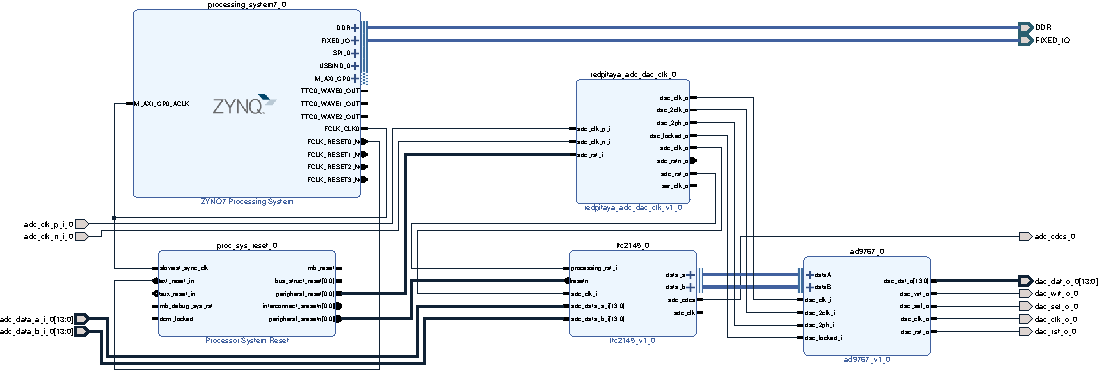
\includegraphics{./block_design.pdf}
\caption{Bloc design comportant le processeur, le bloc de reset, un ADC, un DAC
et le bloc de gestion des horloges pour ces derniers}
\label{bloc_design_final}
\end{figure}


\section{Arborescence}

\begin{lstlisting}
mkdir my_project
mkdir -p my_project/app my_project/modules
\end{lstlisting}

% JMF : je commente, je ne comprends pas ce qu'est cette ligne ci-dessous ni la suite
%vivado settings.me
%\begin{lstlisting}
%VERS=2016.2
%BASE_DIR="/data/Xilinx/Vivado"
%source ${BASE_DIR}/${VERS}/settings64.sh
%export LD_LIBRARY_PATH=${BASE_DIR}/${VERS}/ids_lite/ISE/lib/lin64:$LD_LIBRARY_PATH
%export LANG="en_US.UTF-8"
%\end{lstlisting}

% JMF pour un tuto, je pense qu'on peut se limiter a l'install par default. Le mec qui met dans /data sait se demerder
\begin{lstlisting}
source /opt/Xilinx/Vivado/settings64.sh
vivado
\end{lstlisting}

\section{Cr\'eation du design}

La cr\'eation d'un design pour la {\tt redpitaya} ne comporte pas de
difficult\'es particuli\`eres (\'etapes pr\'esent\'es sur les figures
\ref{createProj1}, \ref{createProj_selectType}, \ref{createProj_selectpart} et
\ref{createProj_summary}),
si ce n'est le fait qu'elle ne soit pas connue,
\`a priori par {\tt Vivado} et qu'il est donc n\'ecessaire de fournir les
caract\'eristiques du Zynq au lieu de choisir la plate-forme (figure
\ref{createProj_selectpart}).

\begin{figure}[h!tb]
\begin{center}
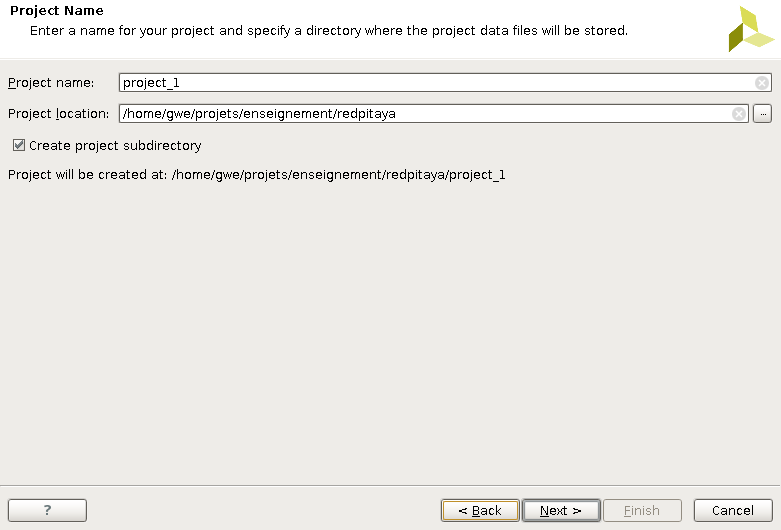
\includegraphics[width=0.5\textwidth]{./createProj1.png}
\end{center}
\caption{Fen\^etre de choix du nom du projet et du r\'epertoire de stockage}
\label{createProj1}
\end{figure}
\begin{figure}[h!tb]
\begin{center}
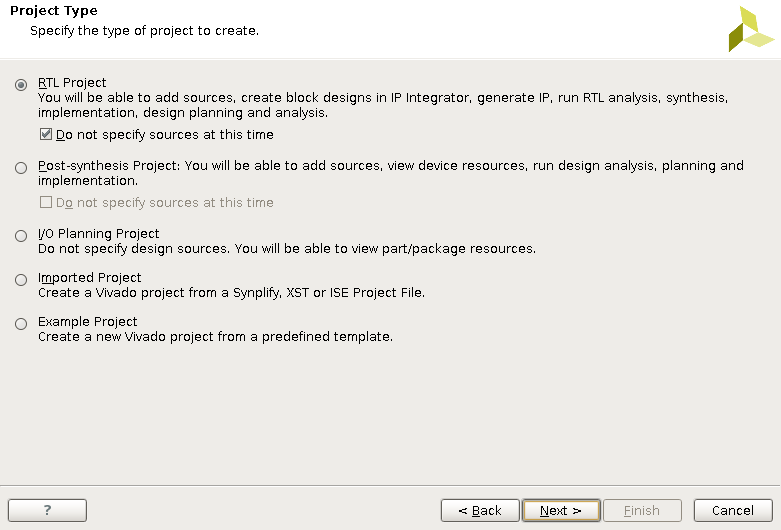
\includegraphics[width=0.5\textwidth]{./createProj_selectType.png}
\end{center}
\caption{Fen\^etre de choix du type de projet. Le choix est {\tt RTL Project}
qui permet de r\'ealiser toutes les manipulations n\'ecessaires. L'option {\em
Do not specify sources at this time} permet d'\'eviter que {\tt Vivado} demande
la liste des fichiers sources lors de la cr\'eation du projet}
\label{createProj_selectType}
\end{figure}
\begin{figure}[h!tb]
\begin{center}
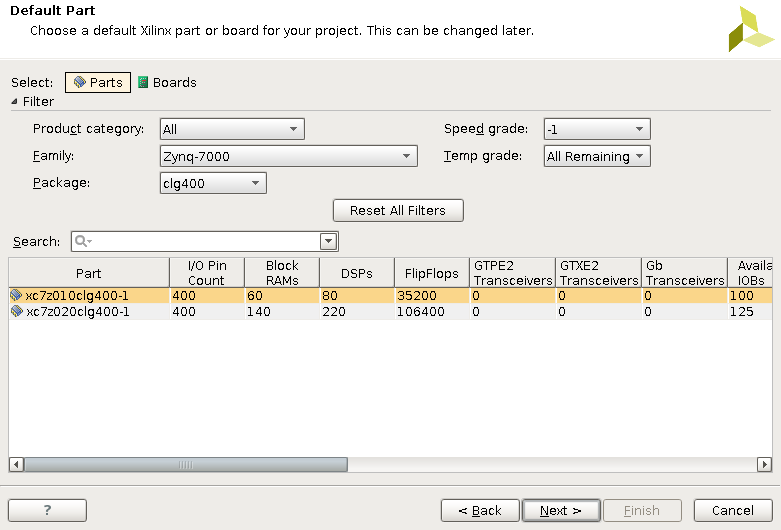
\includegraphics[width=0.7\textwidth]{./createProj_selectPart.png}
\end{center}
\caption{Fen\^etre de choix du mod\`ele du FPGA/Zynq. La redpitaya comporte un
Zynq de type {\tt xc7z010clg400-1} soit
un {\tt Zynq-7000} dans un bo\^\i tier de type {\tt clg400}, avec un {\em speed
grade} valant -1.}
\label{createProj_selectpart}
\end{figure}
\begin{figure}[h!tb]
\begin{center}
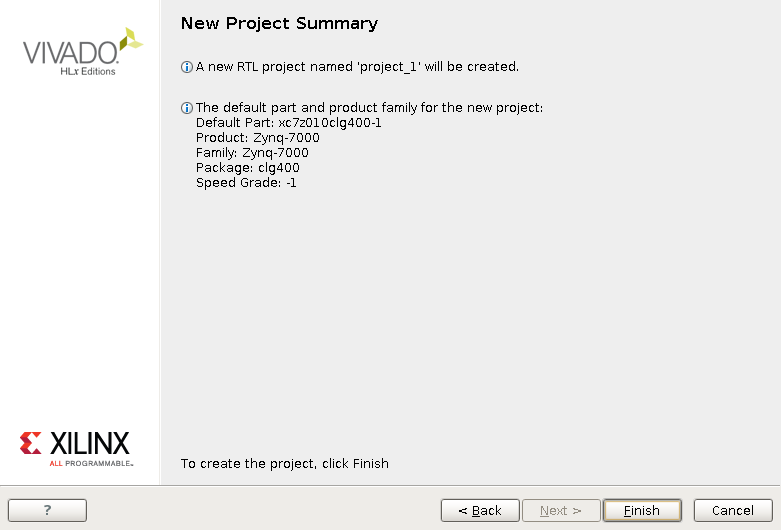
\includegraphics[width=0.5\textwidth]{./createProj_summary.png}
\end{center}
\caption{Fen\^etre r\'ecapitulative.}
\label{createProj_summary}
\end{figure}

\section{Cr\'eation du bloc design}

Dans l'approche la plus classique avec {\tt Vivado}, l'assemblage des {\tt IPs}
se fait de mani\`ere graphique. Ceci se faisant dans le {\em block design}

Dans le menu de gauche, double-cliquer sur {\em Create Block Design}. Le choix
du nom du design n'a pas d'importance mais donnera le nom du bitstream final.
Afin d'avoir une certaine coh\'erence il est pr\'ef\'erable de choisir le m\^eme nom
que le projet.

Le premier \'el\'ement \`a ajouter est le {\em processing system}
(repr\'esentation du processeur dans le {\tt block design}). Ceci se fait
par le raccourci {\tt CTRL + i} pour afficher la fen\^etre de s\'election des
{\tt IPs}. Dans la liste choisir {\em ZYNQ7 Processing System} (mot cl\'e
{\tt zynq} dans la zone de recherche). Sans l'ajout de
ce composant, même s'il n'est n\'ecessaire, le fait de flasher le {\tt FPGA}
depuis {\tt Linux} aura pour effet de bloquer le processeur.

Une fois ce bloc ajout\'e une barre verte appara\^it avec l'option {\em Run
Block Automation}. En appuyant dessus les quelques connexions obligatoires par
d\'efaut seront r\'ealis\'es. 

Comme lors de la cr\'eation de projet, le {\em block design} n'a pas
connaissance des caract\'eristiques particuli\`eres de la {\tt redpitaya} (RAM,
p\'eriph\'eriques, etc.). Afin de disposer d'une base adapt\'ee pour la suite
il est n\'ecessaire de configurer le {\em processing system}. Pour cela en
double cliquant sur ce bloc, en haut de la nouvelle fen\^etre, dans le menu
{\tt Presets}~: choisir {\em Apply configuration} et choisir le fichier {\tt
redpitaya.tcl} se trouvant dans le r\'epertoire {\tt red\_vivado\_support} du
d\'ep\^ot \url{https://github.com/trabucayre/redpitaya/}, ou en local
{\tt fpga\_dev/redpitaya/redpitaya.tcl}.

\section{Configuration de Vivado pour int\'egrer les IPs locales}

{\tt Tools} $\rightarrow$ {\tt Settings} $\rightarrow$ {\tt IP} 
$\rightarrow$ {\tt Repository} $\rightarrow$ {\tt +} et ajouter
{\tt somewhere/fpga\_ip}. Cette op\'eration n'est \`a faire qu'une seule
fois lors de la premi\`ere utilisation des IPs avec une nouvelle installation
de Vivado.

\section{Insertion des blocs dans Vivado}

Dans le bloc design trois composants doivent \^etre ins\'er\'es~:
\begin{itemize}
\item ltc2145~: l'ADC; 
\item redpitaya\_adc\_clk~: Gestion des horloges pour l'ADC et le DAC;
\item AD9767~: le DAC.
\end{itemize}

Comme le design ne comporte pas de communications avec le processeur, certains
blocs ne sont pas ajout\'es. C'est le cas de l'{\em axi interconnect} et du
{\em Processor System Reset}. Le second bloc est toutefois n\'ecessaire dans
notre cas car nous aurons besoin de signaux de reset. Ainsi, apr\`es avoir
fait, \`a nouveau, un {\tt CTRL + i} choisir {\em Processor System Reset} (mot
cl\'e {\tt reset} dans le champ de recherche).

\section{Connexion des blocs sur les broches du FPGA}

Ces trois composants logiciels doivent \^etre, physiquement, connect\'es aux
broches du FPGA (se reporter \`a la figure \ref{bloc_design_final} en cas de
doutes).

Exporter un signal vers l'ext\'erieur se fait \`a l'aide de la commande
{\em make external}~: apr\`es avoir s\'electionn\'e un signal d'un bloc (le
trait et son nom passent en marron) faire un clic-droit et choisir
{\em make external} ou utilisez le raccourci {\tt CTRL + t}.

Les signaux suivant doivent \^etre export\'es~:
\begin{itemize}
\item pour l'ADC~: 
	\begin{itemize}
	\item {\tt adc\_data\_a\_i};
	\item {\tt adc\_data\_b\_i};
	\item {\tt adc\_cdcs}.
	\end{itemize}
\item pour le DAC~:
	\begin{itemize}
	\item {\tt dac\_dat\_o};
	\item {\tt dac\_wrt\_o};
	\item {\tt dac\_sel\_o};
	\item {\tt dac\_clk\_o};
	\item {\tt dac\_rst\_o}.
	\end{itemize}
\item pour le bloc de gestion des signaux d'horloges~:
	\begin{itemize}
	\item {\tt adc\_clk\_p\_i};
	\item {\tt adc\_clk\_n\_i};
	\end{itemize}
\end{itemize}

La commande {\tt make external} (CTRL+t) que nous venons d'effectuer
a permis d'exporter les signaux vers
l'ext\'erieur mais il est \'egalement n\'ecessaire, pour chaque ``fils'', de
d\'efinir \`a quelle broche du FPGA il doit \^etre connect\'e.
Les contraintes de ce type sont fournies dans des fichiers sp\'ecifiques avec une extension
{\tt .xdc}. Pour les trois IPs pr\'esentent dans le {\tt design} ces fichiers
sont fournis dans les r\'epertoires des {\tt IPs} dans le d\'ep\^ot et doivent
simplement \^etre ajout\'es~:
\begin{itemize}
\item dans l'onglet {\tt Sources} \`a gauche de la zone d'assemblage,
d\'erouler {\tt Constraints} et faire un clic-droit sur {\tt constrs\_1}
(figure \ref{addSources}) et s\'electionner {\em Add Sources}
\item {\em Add or create constraints};
\item avec le bouton ``+'', {\em Add Files} et choisir les fichiers {\tt xdc}
	\begin{itemize}
	\item {\tt ad9767.xdc};
	\item {\tt ltc2145-redpy.xdc};
	\item {\tt redpitaya\_clk\_pin.xdc}
	\end{itemize}
	se trouvant dans les r\'epertoires des {\tt IPs} dans le d\'ep\^ot.
\item avant de valider par {\tt Finish}, cocher la case {\em Copy constraints
files into project}. Dans le cas contraire le projet fera r\'ef\'erence aux
fichiers du d\'ep\^ots (en chemin absolu) avec le risque d'erreur si le
d\'ep\^ot est d\'eplac\'e (cas d'un travail colaboratif).
\end{itemize}

\begin{figure}[h!tb]
\begin{center}
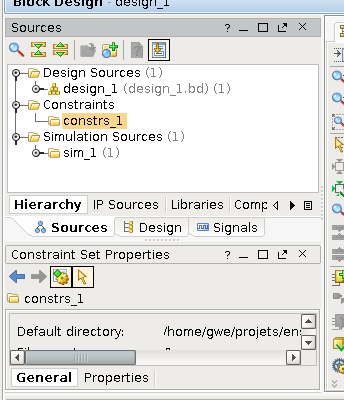
\includegraphics[width=0.4\textwidth]{addSources}
\end{center}
\caption{Ajout des contraintes pour le mapping entre des signaux et des broches
du FPGA}
\label{addSources}
\end{figure}

\section{Connexion des signaux d'horloges et de {\tt reset}}

Pour fonctionner les blocs {\tt ltc2145} et {\tt ad9767} doivent recevoir des
signaux d'horloges et de reset~:

Pour l'ADC~:
\begin{itemize}
\item {\tt processing\_rst\_i} doit \^etre connect\'e sur le signal {\tt
peripheral\_reset} du {\tt Processor system Reset};
\item {\tt resetn} doit \^etre connect\'e sur le signal {\tt
peripheral\_aresetn} du {\tt Processor system Reset};
\item {\tt adc\_clk\_i} doit \^etre connect\'e sur le signal {\tt adc\_clk\_o}
du {\tt redpitaya\_adc\_clk}.
\end{itemize}

Pour le DAC~:
\begin{itemize}
\item {\tt dac\_clk\_i} se connecte sur {\tt dac\_clk\_o} du {\tt
redpitaya\_adc\_clk};
\item {\tt dac\_2clk\_i} se connecte sur {\tt dac\_2clk\_o} du {\tt
redpitaya\_adc\_clk};
\item {\tt dac\_2ph\_i} se connecte sur {\tt dac\_2ph\_o} du {\tt
redpitaya\_adc\_clk};
\item {\tt dac\_locked\_i} se connecte sur {\tt dac\_locked\_o} du {\tt
redpitaya\_adc\_clk}.
\end{itemize}

Sur le g\'en\'erateur d'horloges~:
\begin{itemize}
\item {\tt adc\_rst\_i} de {\tt redpitaya\_adc\_dac\_clk} connecte sur {\tt 
peripheral\_reset} du {\tt proc\_sys\_reset}
\end{itemize}

Connecter la sortie de l'ADC sur l'entr\'ee du DAC~:
\begin{itemize}
\item {\tt data\_a} du ltc2145 se connecte sur {\tt dataA} du {\tt ad9767}
\item {\tt data\_b} du ltc2145 se connecte sur {\tt dataB} du {\tt ad9767}
\end{itemize}

\section{Autres connexions}

Dans le cas de designs comportant de la communication AXI, certaines connexions
sont automatiquement r\'ealis\'ees. Dans le cas pr\'esent celles-ci doivent \^etre
faites manuellement~:
\begin{itemize}
\item le signal {\tt FCLK\_CLK0} du {\tt processing\_system7\_0} doit \^etre
connect\'e~:
	\begin{itemize}
	\item sur le signal {\tt M\_AXI\_GP0\_ACLK} du m\^eme bloc;
	\item sur le signal {\tt slowest\_sync\_clk} du bloc {\tt
	rst\_processing\_system7\_0\_125M}.
	\end{itemize}
\item le signal {\tt FCLK\_RESET0\_N} du {\tt processing\_system7\_0} doit \^etre
connect\'e sur le 
signal {\tt ext\_reset\_in} du bloc {\tt rst\_processing\_system7\_0\_125M}
\end{itemize}

\section{G\'en\'eration du bitstream}

Le projet est maintenant complet, mais avant de pouvoir lancer la
g\'en\'eration du {\tt bitstream} une derni\`ere \'etape est n\'ecessaire~: la
cr\'eation d'un wrapper dont le r\^ole est d'assembler en HDL les divers blocs
dans leur version code. Ce fichier est \'egalement le {\tt top} du design.

Ceci se fait dans l'onglet {\tt Sources} en faisant un clic-droit sur
l'\'el\'ement dont le nom correspond \`a celui du bloc design (figure
\ref{createHDLWrapper}) et en s\'electionnant {\tt Create HDL Wrapper}.

Une fois cette \'etape r\'ealis\'ee il ne reste plus qu'\`a double cliquer sur
le champ {\tt Generate Bitstream} en bas de la zone de gauche de {\tt Vivado}.

\begin{figure}[h!tb]
\begin{center}
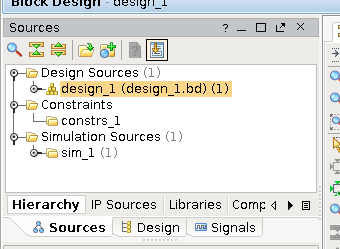
\includegraphics[width=0.5\textwidth]{createHDLWrapper}
\end{center}
\caption{Cr\'eation du wrapper ({\tt top} du design) n\'ecessaire \`a la
g\'en\'eration du {\em bitstream}}.
\label{createHDLWrapper}
\end{figure}

\section{Production d'un bitstream sign\'e et programmation du {\tt FPGA}}

L'\'etape pr\'ec\'edente \`a permis de g\'en\'erer un fichier {\tt .bit}. Celui
se trouve dans le r\'epertoire
{\tt nom\_du\_projet/nom\_du\_projet.runs/impl\_1} et se nomme {\tt nom\_du\_design\_wrapper.bit}
\subsection{G\'en\'eration du fichier crypt\'e}

Vivado g\'en\`ere par d\'efaut un fichier {\tt .bit}.
Le pilote s'attend \`a un autre format contenant un ent\^ete particulier. La conversion
se fait avec l'utilitaire {\tt bootgen} fourni par le SDK de Vivado.

Cet outil attend un fichier .bif contenant~:
\begin{lstlisting}
all:
{
  nom_du_bitstream.bit
}
\end{lstlisting}

qui sera ensuite fourni \`a {\tt bootgen}~:
\begin{lstlisting}[language=bash]
$VIVADO_SDK/bin/bootgen -image fichier_bif.bif -arch zynq -process_bitstream bin
\end{lstlisting}

Suite \`a cette commande un fichier {\tt nom\_du\_bitstream.bit.bin} est cr\'e\'e
dans le r\'epertoire courant.

\subsection{Flasher par utilisation directe de {\tt fpga\_manager}}

Le fichier {\tt .bit.bin} doit \^etre copi\'e/d\'eplac\'e dans {\tt /lib/firmware}.

Afin d'informer le pilote que le {\tt PL} doit \^etre flash\'e, et quel
bitstream utiliser, la commande suivante est \`a utiliser~:
\begin{lstlisting}[language=bash]
echo "nom_du_bitstream.bit.bin" > /sys/class/fpga_manager/fpga0/firmware
\end{lstlisting}
La ligne~:
\begin{lstlisting}[language=bash]
fpga_manager fpga0: writing nom_du_bitstream.bit.bin to Xilinx Zynq FPGA Manager
\end{lstlisting}
s'affichera en cas de succ\`es et la LED connect\'ee sur {\tt Prog done} doit
s'allumer (LED bleue sur la {\tt RedPitaya}).

\subsection{Utilisation d'un overlay pour le {\tt devicetree} pour le flashage}

Comme pour l'autre solution, le bitstream doit se trouver dans
{\tt /lib/firmware}.

L'int\'er\^et de cette m\'ethode par rapport \`a la pr\'ec\'edente est que lorsque
le design contient des IPs qui communiquent avec le processeur, le {\em devicetree}
communique au noyau les informations requises par les pilotes.
G\'en\'eralement dans ce type de cas un pilote est disponible et celui-ci doit
\^etre charg\'e. L'overlay permet, par surcharge et ajout, de fournir, \`a la
fois, le nom du
bitstream, et de compl\'eter le devicetree charg\'e au d\'emarrage
avec les pilotes sp\'ecifiques \`a l'application.

Sans rentrer dans tous les d\'etails de ce type de fichier, le code suivant \`a
pour r\^ole de~:
\begin{itemize}
\item modifier le n\oe ud {\tt fpga\_full} (attribut {\tt target}), correspondant au {\tt fpga\_manager}
	pour lui fournir le nom du binaire \`a charger au travers de l'attribut
	{\tt firmware-name};
\item d'ajouter des sous-n\oe uds correspondant aux pilotes n\'ecessaires afin
de permettre leur chargement. Dans le cas pr\'esent le pilote associ\'e est
{\tt gpio\_ctl} (champ {\tt compatible}), et on fournie l'addresse de base sur
la plage m\'emoire partag\'ee entre le PS et le PL (0x43C00000), la taille de
la zone (0x1f) par l'attribut {\tt reg}
\end{itemize}\vspace{0.3cm}
 
\begin{lstlisting}
/dts-v1/;
/plugin/;
/ {
    compatible = "xlnx,zynq-7000";
    fragment@0 {
        target = <&fpga_full>;
        #address-cells = <1>;
        #size-cells = <1>;
        __overlay__ {
            #address-cells = <1>;
            #size-cells = <1>;

            firmware-name = "top_redpitaya_axi_gpio_ctl.bin";

            gpio1: gpio@43C00000 {
                compatible = "gpio_ctl";
                reg = <0x43C00000 0x0001f>;
                gpio-controller;
                #gpio-cells = <1>;
                ngpio= <8>;
            };
        };
    };
};

\end{lstlisting}

Ce fichier doit ensuite \^etre compil\'e par la commande~:
\begin{lstlisting}
/somewhere/buildroot/output/host/usr/bin/dtc -@ -I dts -O dtb -o ${FILENAME}.dtbo ${FILENAME}.dts
\end{lstlisting}
Avec~:
\begin{itemize}
\item {\tt -@} pour la g\'en\'eration de symboles qui seront dynamiquement
li\'es lors du chargement dans la m\'emoire;
\item {\tt -I dts} pour d\'efinir le type du fichier d'entr\'ee;
\item {\tt -O dtb} pour d\'efinir le type du fichier de sortie;
\item {\tt -o} le nom du fichier g\'en\'er\'e.
\end{itemize}

Pour charger le fichier en m\'emoire deux \'etapes sont n\'ecessaires~:
\begin{enumerate}
\item
la cr\'eation d'un r\'epertoire correspondant \`a notre overlay~:
\begin{lstlisting}[language=bash]
mkdir /sys/kernel/config/device-tree/overlays/toto
\end{lstlisting}
se traduira par la cr\'eation automatique d'un ensemble de
fichiers qui peuplera ce r\'epertoire~:
\begin{lstlisting}[language=bash]
redpitaya> ls -l /sys/kernel/config/device-tree/overlays/toto/
total 0
-rw-r--r--    1 root     root             0 Jan  1 00:04 dtbo
-rw-r--r--    1 root     root          4096 Jan  1 00:04 path
-r--r--r--    1 root     root          4096 Jan  1 00:04 status
\end{lstlisting}
\item
le chargement de l'overlay dans le {\em devicetree}~:
\begin{lstlisting}[language=bash]
cat gpio_red.dtbo > /sys/kernel/config/device-tree/overlays/toto/dtbo
\end{lstlisting}
induira la configuration du FPGA par transfert du bitstream, activation du pilote associ\'e
\`a cet overlay par la m\'ethode ``compatible'' qui aura \'et\'e renseign\'ee dans le champ appropri\'e
du module.
\end{enumerate}
 
Il est \'egalement possible d'annuler les modifications (revenir \`a l'\'etat
initial) en supprimant le r\'epertoire~:
\begin{lstlisting}[language=bash]
rm -rf /sys/kernel/config/device-tree/overlays/toto
\end{lstlisting}
\end{document}
